\documentclass[11pt]{amsart}
\usepackage[margin=1in]{geometry}
\usepackage{graphicx}
\usepackage{siunitx}
\usepackage{amsmath,amsfonts,amsthm,amssymb,amsaddr}
\usepackage{hyperref}
\usepackage{fancyhdr}
\usepackage{multicol, caption}
\usepackage[font=small,labelfont=bf]{caption}

\graphicspath{ {./images/} }

\setlength{\headheight}{11pt}

%\makeatletter
%\def\subsection{\@startsection{subsection}{3}%
%  \z@{.5\linespacing\@plus.7\linespacing}{.1\linespacing}%
%  {\normalfont\itshape}}
\newenvironment{Figure}
  {\par\medskip\noindent\minipage{\linewidth}}
  {\endminipage\par\medskip}
%\makeatother

\title{Observation of the Higgs Boson in the $H \to \gamma\gamma$ Channel from Data Simulated in Pythia}

\author{Joe Bentley}

\address{School of Physics and Astronomy \\ Tutor: Kevin Ralley}
\email{joebentley10@gmail.com}

\date{\today}

\begin{document}

\begin{abstract}
  In this paper the higgs data is analysed and we find the higgs with this statistical significance etc.
\end{abstract}

\maketitle

\newpage

\pagestyle{fancyplain}

\lhead{\footnotesize {Joe Bentley}}
\rhead{\footnotesize {Lab Report}}

\begin{multicols}{2}

\section{Introduction}

In this experiment particle collision data is analysed using multiple Python scripts to generate an invariant mass histogram and attempt to find the Higgs boson with some statistical significance in the mass window $\SI{115}{\giga\electronvolt}$ to $\SI{135}{\giga\electronvolt}$. In real high energy physics experiments, an observation is only accepted when the excess of events observed is more than 5 standard deviations ($5\sigma$) away from the expected background count. \cite{5sigma} The collision data is generated in PYTHIA as a flat text file containing the four momenta of photons in the detector, which is parsed by the parsing script which filters the events to give the best statistical significance for the Higgs and calculates the invariant masses as described in section ~\ref{sec:invariant}. These invariant masses are then counted and put into bins to create an invariant mass histogram.

The difficulty in this experiment is due to a number of factors. First there is very little Higgs signal compared to the background, because the Higgs production cross section and branching fraction of the decay mode we are interested in (see section ~\ref{sec:branching}) are much smaller than the background cross section. The Higgs signal is indistinguishable in the unfiltered mass range without significant filtering to try and reduce the background.

The experiment is interesting as it relies on our ability to constantly improve our results, instead of setting up the equipment and taking the first few sets of results. Our first results are unusable as they are unfiltered, so the experiment relies on our ability to iterate our filtering techniques to find the most effective methods. A process that was automated to some degree in section ~\ref{sec:optimisation}.

\section{Theory}

\subsection{Four Momentum}
\label{sec:fourmomentum}

The four momentum is similar to the classical three component momentum except generalised to four dimensional space-time, so it also has an energy component. \cite{kinematics} In the data supplied the four-momentum is given in the form $(p_x, p_y, p_z, E)$, where $p_z$ is aligned along the beam axis

The transverse momentum is the component of the momentum perpendicular to the beam axis. Since the $z$ component of the four-momentum, $p_z$ is aligned along the beam axis, the transverse momentum is given by,

\begin{equation}
  \label{eq:transverse}
  p_T = \sqrt{{p_x}^2 + {p_y}^2}.
\end{equation}

The pseudorapidity is a measure of the polar angle $\theta$, the angle between the particle and the beam axis, and is defined as,

\begin{equation}
  \label{eq:pseudorapdity2}
  \eta = -\ln{\left[\tan{\left(\frac{\theta}{2}\right)}\right]} = \frac{1}{2}\ln{\left(\frac{|\mathbf{p}|+p_z}{|\mathbf{p}|-p_z}\right)},
\end{equation}

\cite{kinematics}

which can be calculated from the cartesian momentum components of the four momenta used in this experiment by,

\begin{equation}
  \label{eq:pseudorapidity}
  \eta = \sinh^{-1} \frac{p_z}{p_T}.
\end{equation}

The rapidity is given by,

\begin{equation}
  \label{eq:rapidity}
  y = \frac{1}{2}\ln{\left(\frac{E + p_z}{E - p_z}\right)},
\end{equation}

which in our case is equal to the pseudorapidity, as we are measuring photons which have zero rest mass, hence $E = |\mathbf{p}|$.

The azimuthal angle is the angle between the momentum and the $x$-axis as seen in the $xy$-plane, in contrast to the pseudorapidity, which is between the particle trajectory and the beam axis (see fig.~\ref{fig:kinematics}),

\begin{equation}
  \label{eq:azimuthal}
  \phi = \tan^{-1} \frac{p_y}{p_x}.
\end{equation}

It can also be thought of the angle between the $x$-axis and the transverse momenta \textit{vector}, which is just $\mathbf{p_T} = (p_x, p_y, 0)$, the momentum projected onto the $xy$-plane.

A lorentz invariant quantity measure of angular seperation which is a combination of pseudorapidity and azimuthal angle can also be defined,

\begin{equation}
  \label{eq:angular}
  {(\Delta R)}^2 = {(\Delta \eta)}^2 + {(\Delta \phi)}^2.
\end{equation}

The quantity $\Delta R$ is Lorentz invariant because both the difference in pseudorapidity $\Delta \eta$ and difference in azimuthal angle $\Delta \phi$ are Lorentz invariant. \cite{lorentz}

\begin{Figure}
  \centering
  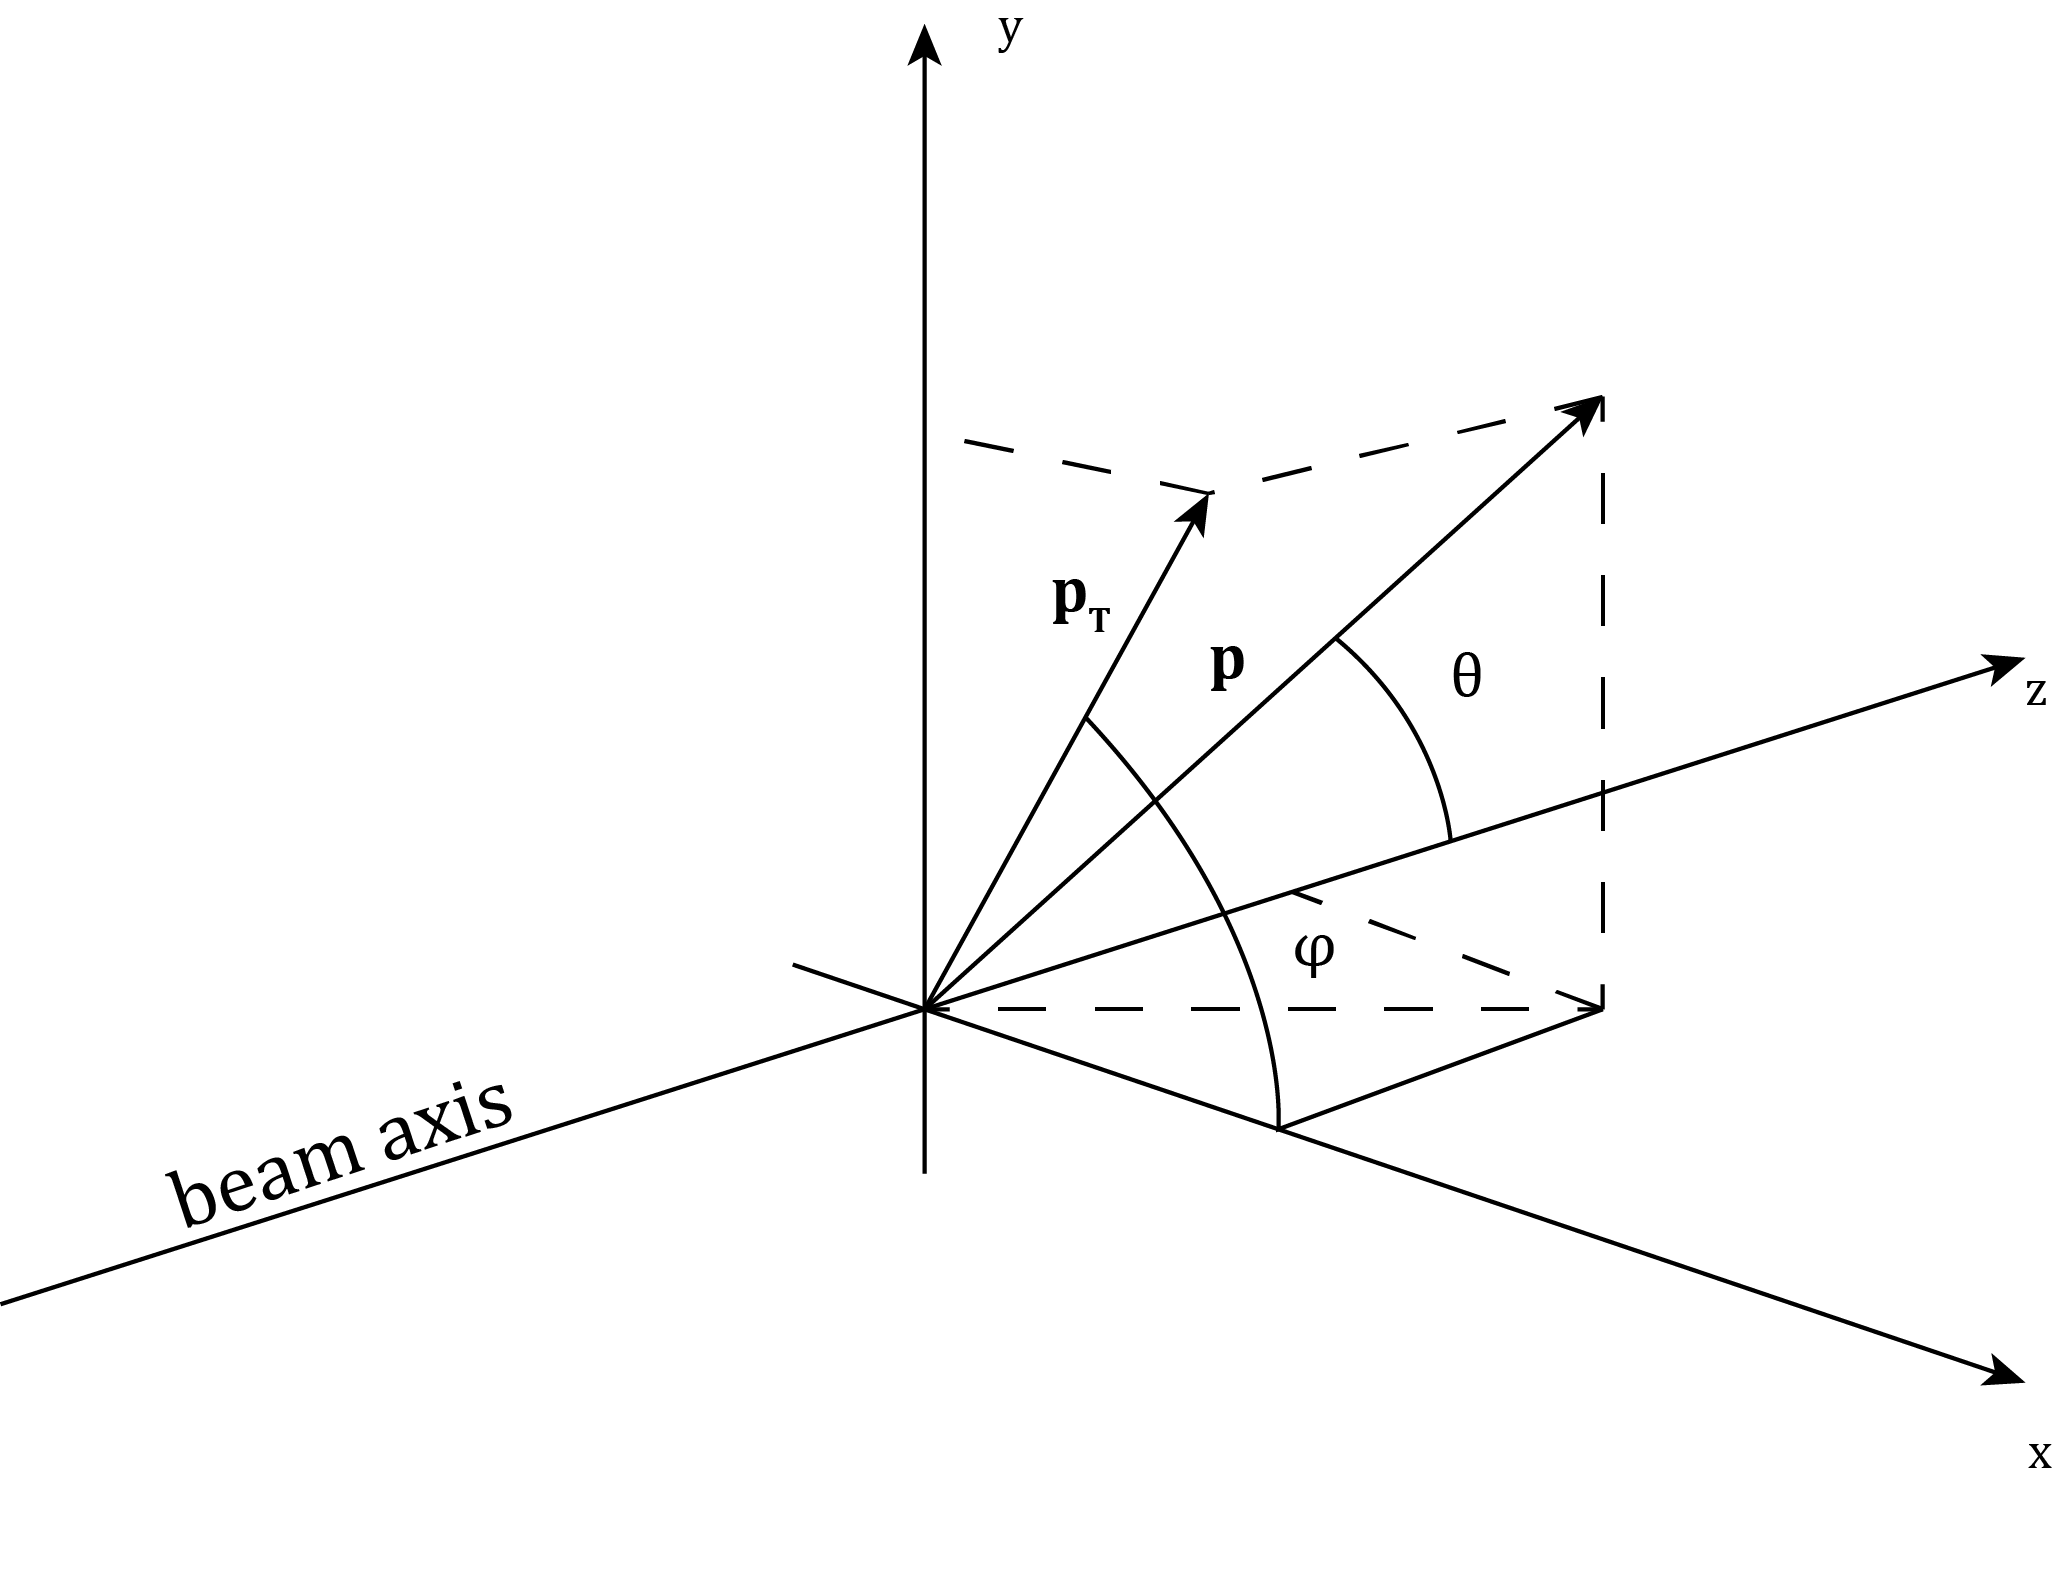
\includegraphics[width=\linewidth]{kinematics}
  \captionof{figure}{A diagram showing the transverse momenta $p_T$, the azimuthal angle $\phi$, and the polar angle $\theta$ in the case where the beam axis is aligned with the $z$-axis}
  \label{fig:kinematics}
\end{Figure}

\subsection{Branching Fraction}
\label{sec:branching}

The branching fraction is the fraction of all particles which decay through a given decay mode, in this case the ratio of number of Higgs that decay through $H \to \gamma\gamma$ to the number that decay through all decay modes for a given number of Higgs decaying. For example, if the branching fraction for a given decay mode is $0.5$, then on average half of the particles will decay through that mode.

\subsection{Higgs Decay Channels}

Since the Higgs is a very massive particle, it can decay through a large number of different decay modes: (GET SOURCE)

\begin{itemize}
    \item Fermion-antifermion pair
    \item Pair of massive gauge bosons
    \item Pair of massless gauge bosons (through heavy virtual quark or massive gauge boson loop)
\end{itemize}

\cite{decaymodes1} \cite{decaymodes2}

(MAYBE A BIT MORE EXPLANATION ABOUT THESE DECAY MODES?! (GET ANOTHER SOURCE?!)

The decay channel investigated in this experiment is the last one, the decay of the Higgs into two photons by a heavy virtual quark (top) or massive gauge boson (W boson) loop. This is significantly rarer than the other decay modes as seen in the small branching fraction of 0.0023 (so it occurs twice in every thousand decays) \cite{HiggsCross1}, but is used because the momenta of the photons can be measured much more accurately than other more massive particles, since the momenta of the photon is directly proportional to its energy, as the photon has no rest mass. (GET SOURCE) (HOW TO MEASURE PARTICLE MOMENTUM? LOOK AT ATLAS EXPERIMENT)

\subsection{Invariant Mass}
\label{sec:invariant}

To find the mass of the particle(s) before a collision event, the invariant mass is used, which is the mass which remains unchanged through a Lorentz transform (GET SOURCE). The sum of the invariant masses of the products of an interaction is the same as the sum of the invariant masses of the original particles, so by calculating the sum of the invariant masses of the resultant particles of the collision events, we have calculated the sum of the invariant masses of the inputs of the collision event. In our case this invariant mass corresponds to either the background, or the Higgs on its own.

The invariant mass is calculated using the relativistic equation for energy, in natural units this is given by,

\begin{equation}
  \label{eq:invariantmass}
  m_0^2 = E^2 - {|\mathbf{p}|}^2
\end{equation}

This is calculated in the parsing program by summing the four momenta from the event and then taking the scalar product of the resulting vector with itself. Minkowski space-time has signature $(+, -, -, -)$ so the scalar product has the effect of the above equation. We then take the square root of the scalar product to find the invariant mass. \cite{kinematics}

The mass window we are observing is taken to be $\SI{115}{\giga\electronvolt}$ to $\SI{135}{\giga\electronvolt}$, which is roughly $\pm \SI{10}{\giga\electronvolt}$ the expected Higgs mass, as measured. \cite{Higgs}

\subsection{Statistics}

Since this is a counting experiment where the number of events counted is independent (the number of events counted in one time interval has no effect on the number of events counted in the next time period) the experiment obeys Poisson statistics. In Poisson statistics the variance is equal to the number of events counted in the time interval $\lambda$ such that $\sigma^2 = \lambda$. The mean number of events $\lambda$ in this case is just the number of events counted, $\lambda = S + B$ where $S$ is the number of signal (Higgs) events, and $B$ is the number of background events. This means that the standard deviation is given by taking the square root of the variance $\sigma = \sqrt{\lambda} = \sqrt{S + B}$. (GET SOURCE ON POISSON STATISTICS)

The statistical significance is a measure of how many standard deviations a result (being the number of counts observed in excess of the expected amount, the mean) lies away from the expected value, so is given by $\frac{S}{\sigma}$, where $S$ is the observed excess (in this case the number of signal events) and $\sigma$ is the standard deviation. Since $\sigma = \sqrt{S + B}$ statistical significance is therefore given by,

\begin{equation}
  \label{eq:significance}
  \Sigma = \frac{S}{\sqrt{S + B}}
\end{equation}

\section{PYTHIA}
\label{sec:pythia}

The GPL-licensed PYTHIA was used to generate the collision data used in this experiment. \cite{pythia} The event data is given in a flat text file format. The file consists of a series of events, which start with a header ``Event $n$'', the subsequent lines are the four momenta of the products of the collision event, each line in the format ``$p_x$ $p_y$ $p_z$ $E$'', where $p_z$ is aligned along the beam axis. Then there is another line ``Event $n+1$'' with subsequent lines being four momenta events and so on.

\section{Programming}

The scripts used in this experiment were written in Python 3, and used the numpy (numeric Python) module for generating the histogram, and PyPlot (from matplotlib) for plotting the histogram and significance plots. Three different scripts were created for this experiment,

\subsection{parse.py}

The script parse.py parses the event data in the format described in section ~\ref{sec:pythia} into individual event objects which each contain a list of four momenta objects. In these event classes we have methods which do useful operations like calculating the invariant mass of the event from the four momenta. The four momenta class has methods that calculate the transverse momentum, azimuthal angle, and pseudorapidity, as well as allowing us to add and take the dot product of four momenta. The parsing script also contains the filters which are used to filter out Higgs events from background events, and are discussed in more depth in section ~\ref{sec:filters}. The invariant masses are calculated for each event in the event data file, and then the resulting list of invariant masses is saved using python's built-in pickle module, which saves python objects in a binary representation, saving space and improving read and write times of the invariant masses.

\subsection{significance.py}

This script optimises the filters used on the Higgs and background data by using a series of parameters with the filters and testing them on the entire data set; the significance is taken for the parameters and this is used to find the best filter parameters, as discussed in section ~\ref{sec:optimisation}. It parses and filters the data using the parsing module.

\subsection{plot.py}

The plotting script generates the histogram of both the higgs and background event data together, called the combined mass histogram. The significance in the mass window ($\SI{115}{\giga\electronvolt}$ to $\SI{135}{\giga\electronvolt}$) is calculated by counting the number of Higgs events in the mass window and the number of background events in the mass window and then using eq.~\ref{eq:significance} to calculate the statistical significance. The script can also generate an invariant mass plot from the combined mass histogram.

\subsection{Testing}
\label{sec:testing}

Python's unit testing framework, unittest, was used to run testing scripts on the filters to ensure that they were working as intended. The tests took a pre-generated dataset and then ran this against each filter, checking the result to see if it is what was expected. This allowed us to debug a major issue in the second transverse momenta filter which is discussed further in section ~\ref{sec:issues}.

\section{Weighting}

The data given included $10,000$ signal events and $1,000,000$ background events. This is a much larger ratio of signal to background events than would actually be observed in a real experiment due to the low branching fraction of the $H \to \gamma\gamma$ decay mode. The theoretical ratio of the observed Higgs events to observed background events can be calculated by taking the ratio of the Higgs production cross section to the background cross section and multiplying it by the branching fraction of $H \to \gamma\gamma$,

\begin{equation}
  \label{eq:weighting}
  \frac{S}{B} = \frac{\sigma_H \cdot B_f\left(H\to\gamma\gamma\right)}{\sigma_B}
\end{equation}

where $S$ is the expected number of signal events, $B$ is the number of background events, $\sigma_H$ is the Higgs production cross section, $\sigma_B$ is the background cross section, and $B_f\left(H\to\gamma\gamma\right)$ is the branching fraction of Higgs to diphoton.

The branching fraction for Higgs to two photons is given by $B_f\left(H\to\gamma\gamma\right) = 0.0023$, and the cross sections are given by $\sigma_H = \SI{17.12}{\pico\barn}$, and $\sigma_B = \SI{140}{\pico\barn}$. The Higgs cross section and branching fraction are taken at roughly the expected Higgs mass $\SI{125}{\giga\electronvolt}$, \cite{Higgs} where the cross section is taken from the ABPS calculation for $\sqrt{s} = \SI{14}{\tera\electronvolt}$ where $s$ is the centre-of-momentum energy (the energy in the frame where the total momenta is zero). \cite{HiggsCross1} \cite{COMframe} (MORE JUSTIFICATION NEEDED). The background cross section is taken from the PYTHIA collision event generator.

\section{Filters}
\label{sec:filters}

There are many more background events than there are from the signal (Higgs) events in our data. After the weighting, there are roughly $100$ Higgs events to $100,000,000$ background events, so in the combined invariant mass histogram the Higgs is practically invisible. Thus filtering needs to be applied for there to be any chance to be able to observe the Higgs in the invariant mass histogram. This is implemented in the form of event selection in which we attempt to remove the background data while retaining the Higgs data. A few types of filtering are used: number threshold, transverse momenta, energy, angular (azimuthal and pseudorapidity).

\subsection{Number}

The first filter applied a threshold to the number of four momenta in the collision event. It is required that the event must have at least two four momenta, as the $H \to \gamma\gamma$ will produce at least two photons, not just one. This filter should have a good effect to clean up a large amount of data which is definitely background, as we know that all events with one four momenta must be background.

\subsection{Transverse Momenta}

The transverse momenta is the component of the momentum perpendicular to the beam axis as described in section ~\ref{sec:fourmomentum}. The filter is applied in two passes over both the signal and background events. First the given event is discarded \textit{unless} it has at least one four momentum with a transverse momentum above a given threshold, denoted $p_1$. Then all four momenta in the event with tranverse momenta below a given threshold, denoted $p_2$, are removed from the event.

(JUSTIFICATION)

\subsection{Energy}

The energy of the four momenta is filtered similarly to how the transverse momenta is filtered. First the event is discarded \textit{unless} it has at least one four momenta with an energy greater than a given threshold, denoted $E_1$. Then all four momenta with an energy less than a given threshold, denoted $E_2$, are removed from the event.

\subsection{Angular}

The square of the difference in azimuthal angle and square of the difference in pseudorapidity are also filtered by finding the maximum difference squared in both the azimuthal and pseudorapidity for all the four momenta in an event. If the maximum difference squared of a given event is below a given threshold, for azimuthal denoted ${(\Delta \phi)}^2$ and for pseudorapidity denoted ${(\Delta \eta)}^2$, then that event is discarded.

\subsection{Final Selection}

There are two methods that were proposed to choose the final two transverse momenta to use to calculate the invariant mass. First it was decided to try an azimuthal angle based filter, where the most back-to-back photons (the photons with an azimuthal angle with the greatest difference) would be chosen to calculate the invariant mass. (WHY DIDN'T YOU DO THIS?!?) Instead all but the two highest transverse momenta photons are discarded, and the two remaining are used to calculated the invariant mass.


\section{Optimisation of Filters}
\label{sec:optimisation}

\begin{Figure}
  \centering
  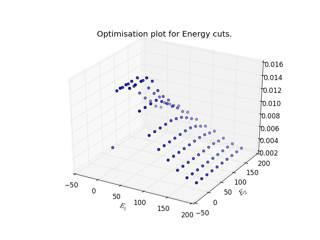
\includegraphics[width=\linewidth]{energy}
  \captionof{figure}{Optimisation plot for the energy, showing the best (highest) values of $E_1 = \SI{40}{\giga\electronvolt}$ and $E_2 = \SI{60}{\giga\electronvolt}$}
  \label{fig:energy}
\end{Figure}

The filters available can be used to attempt to isolate the Higgs signal from the background signal to increase the Higgs statistical significance in the mass window. Without optimising the filter parameters the best parameters to choose are unknown, and so it is just guessing to choose any. By optimising the filters the best possible values are attained. The filter parameters ``goodness'' were measured using the statistical significance from eq.~\ref{eq:significance}.

Each filter is applied to the signal (Higgs) and background events and then the above equation is used to find the statistical significance of the Higgs in those events by counting the number of signal and background events left after filtering. The filter parameters giving the highest statistical significance of the Higgs correpond to filtering out more background than Higgs.

To find the best parameters to use for the filters a range of different parameters are tested for each filter. For example for the transverse momenta filter, the threshold is originally applied from $\SI{0}{\giga\electronvolt}$ to $\SI{700}{\giga\electronvolt}$ in steps of $\SI{100}{\giga\electronvolt}$. The value that gives the best statistical significance is then chosen as the current candidate for the best optimised value. Then the value is further optimised by taking the currently best optimised value and then calculating the statistical significance for the values around it, for example checking the statistical significance at $\SI{\pm10}{\giga\electronvolt}$ the current value for the above example. After repeating this process a few times (HOW MANY TIMES?) the most optimum filter values to give the best statistical significance.

The script also generates 3D scatter plots where the $x$ and $y$-axes correspond to the different filter parameter settings. The $z$-axis (height) of the point correponds to the statistical significance of the Higgs over the entire mass range with those two filter parameters used. Examples of statistical significance plots are figures ~\ref{fig:energy} and ~\ref{fig:transverse}.

After running repeated optimisations over the range \SI{0}{\giga\electronvolt} to \SI{700}{\giga\electronvolt}, the optimum cut values for transverse momenta were found to be $p_1 = \SI{70}{\giga\electronvolt}$ and $p_2 = \SI{90}{\giga\electronvolt}$, and for energy were found to be $E_1 = \SI{40}{\giga\electronvolt}$ and $E_2 = \SI{60}{\giga\electronvolt}$.

\begin{Figure}
  \centering
  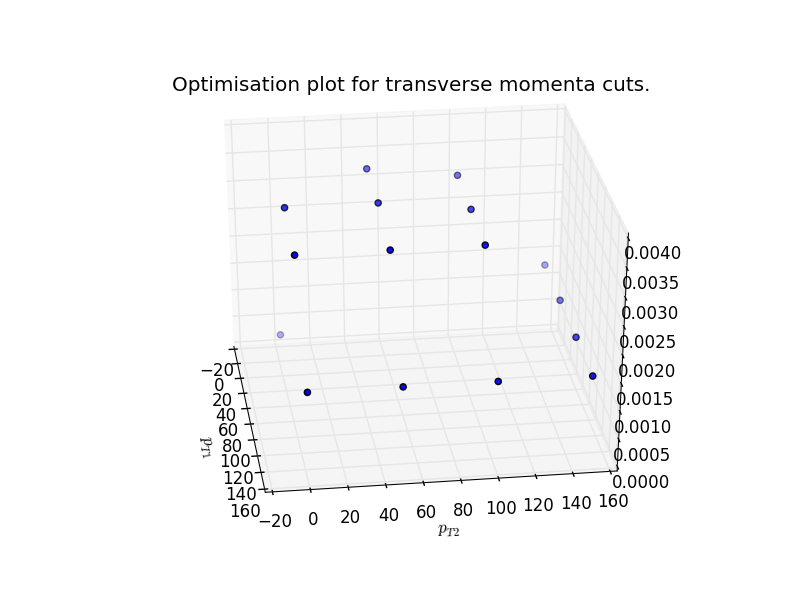
\includegraphics[width=\linewidth]{transverse}
  \captionof{figure}{An optimisation plot for transverse momenta}
  \label{fig:transverse}
\end{Figure}


\section{Invariant Mass Histogram}

The numpy library is used to generate an combined (signal and background) invariant mass histogram from the invariant masses calculated in the parsing script. The statistical significance of the signal (Higgs) is calculated using eq.~\ref{eq:significance} over the mass window discussed in section ~\ref{sec:invariant} by generating a histogram of the Higgs from the Higgs invariant masses, and the same for the background, and then summing the number of signal events and background events found in the mass window ($\SI{115}{\giga\electronvolt}$ to $\SI{135}{\giga\electronvolt}$).

\begin{Figure}
  \centering
  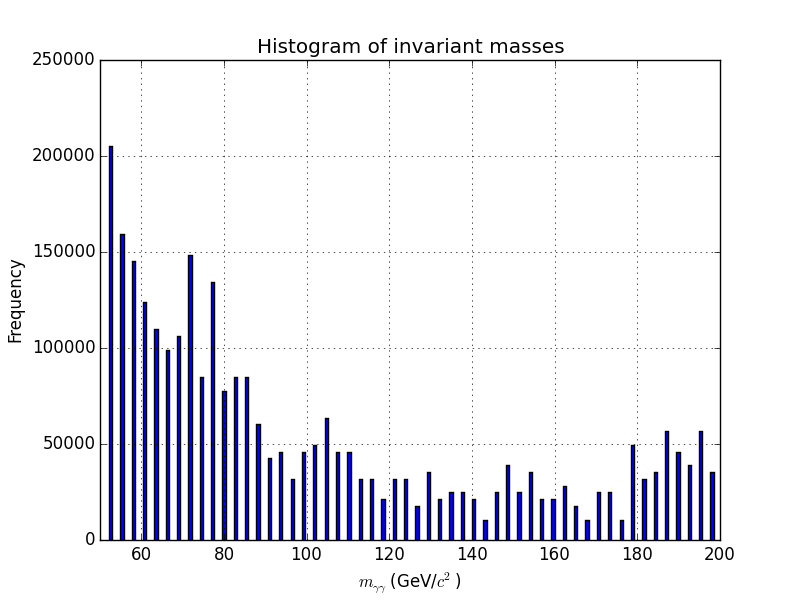
\includegraphics[width=\linewidth]{invmass2}
  \captionof{figure}{Combined invariant mass plot in the range \SI{50}{\giga\electronvolt} to \SI{200}{\giga\electronvolt} with optimised filter parameters applied. In the mass window ($\SI{115}{\giga\electronvolt}$ to $\SI{135}{\giga\electronvolt}$) the Higgs had a significance of $\Sigma = 0.33$}
  \label{fig:invmass}
\end{Figure}

(TALK ABOUT HISTOGRAM RESOLUTION)

\section{Results}

The Higgs was observed in the mass window ($\SI{115}{\giga\electronvolt}$ to $\SI{135}{\giga\electronvolt}$) with a statistical significance of $\Sigma = 0.33$, which was calculated using eq.~\ref{eq:significance}. This means that our observed excess of Higgs was about 0.3 standard deviations from the expected value with just the background. This isn't a conclusive enough result to claim that the Higgs is seen in that mass window. The convention in high energy physics is that a statistical significance of $5 \sigma$ is required to claim that an observation is not just due to chance. \cite{5sigma}

The optimisation of the filters was successful in improving our filtering of the data set. Pre-filtering the data set had a statistical significance of roughly $0.01$, whereas after optimising and applying our filters we obtained a statistical significance of $0.33$, which is a definite improvement.

\section{Issues}
\label{sec:issues}

There were a few issues encountered upon the way. Some were expected but a couple were not, and were harder to fix.

The clearest and most pressing issue was having to filter, since the Higgs was practically invisible in the unfiltered invariant mass plot (having a statistical significance of only $\Sigma = 0.01$). Filters were used to attempt to remove the non-Higgs events from the dataset as discussed in section ~\ref{sec:filters}. Then the most optimum parameters had to be found that would give us the best ratio of signal to background events, as discussed in section ~\ref{sec:optimisation}.

When the invariant mass histogram was generated after finding some preliminary optimised parameters, invariant masses were being repeated. This was revealed by testing as discussed in section ~\ref{sec:testing}, and was due to a missing break statement. These events were being added multiple times in the second transverse momenta and second energy filters (section ~\ref{sec:filters}). The filter would iterate over each four momenta in an event, and if the transverse momentum/energy of the four momentum was greater than the threshold, that event would be added to the list of events to return from the filter. The missing break statement meant that even if a transverse momentum/energy above the threshold was found, the filter would continue to iterate through the event, repeatedly adding the same event to the output list. This was noticed when looking at the invariant mass histogram, there would be some bins that were much taller than adjacent ones, instead of a roughly homogenous distribution. This was due to those bins containing events with \textit{many} four momenta over the transverse momenta/energy threshold, so those events would be added to the invariant mass histogram many more times. This was all fixed by adding a single break statement after a four momentum above the threshold was found, preventing the repeated adding.

Another issue, while not as urgent, was that the parsing script took a very long time to parse all the data. This was due to the entire remainder of the data file being passed to the parsing function every time an event was found, as the file would parse each line as a four momentum until it found another ``Event n'' heading. To fix this a file was created alongside the event data files containing the number of four momenta in each event. This meant that only the number of lines needed were passed to the event parser, instead of all the lines being passed, so instead of having to pass almost a million lines, only around ten lines would need to be passed for each event, which was significantly faster. Without this the parsing script would take many hours to run. Parallel processing from Python's multiprocessing library was also used for a small performance gain.

\section{Conclusion}

\section{Acknowledgments}

Thank you to my lab partner Jake, who did a lot of work on the statistical significance, and was very knowledgable about the topic of the experiment. Thanks to our supervisor Timothy Williams as well for being extremely helpful in any questions we had, as well as pushing us in the right directions. Special thanks to the PYTHIA team for creating great open-source software, and finally to everyone at CERN for making this possible in the first place, as well as doing great things for our understanding of the universe.


\end{multicols}

\bibliographystyle{plain}
\bibliography{citations}
\end{document}
